%%
%% Toolbox Language Manual
%% $Id: m4lib.tex,v 1.33 2006/04/19 10:25:12 vdmtools Exp $
%% 

%%%%%%%%%%%%%%%%%%%%%%%%%%%%%%%%%%%%%%%%
% PDF compatibility code. 

\makeatletter
\newif\ifpdflatex@
\ifx\pdftexversion\@undefined
\pdflatex@false
%\message{Not using pdf}
\else
\pdflatex@true
%\message{Using pdf}
\fi

\newcommand{\latexpdf}[2]{
  \ifpdflatex@ #1
  \else #2
  \fi
}

\newcommand{\latexorpdf}[2]{
  \ifpdflatex@ #2
  \else #1
  \fi
}

\makeatother

#ifdef A4Format
\newcommand{\pformat}{a4paper}
#endif A4Format
#ifdef LetterFormat
\newcommand{\pformat}{letterpaper}
#endif LetterFormat

%%%%%%%%%%%%%%%%%%%%%%%%%%%%%%%%%%%%%%%%

\latexorpdf{
\documentclass[\pformat,12pt]{article}
}{
% pdftex option is used by graphic[sx],hyperref,toolbox.sty
\documentclass[\pformat,pdftex,12pt]{article}
}

\usepackage{toolbox}
\usepackage{rotating}
\usepackage{verbatimfiles}
\usepackage{alltt}
%\usepackage{path}
\usepackage{longtable}

% Ueki change start
\usepackage[dvipdfm,bookmarks=true,bookmarksnumbered=true,colorlinks,plainpages=true]{hyperref}
% Ueki change end

% Ueki delete start
%\latexorpdf{
%\usepackage[plainpages=true,colorlinks,linkcolor=black,citecolor=black,pagecolor=black, urlcolor=black]{hyperref}
%}{
%\usepackage[plainpages=true,colorlinks]{hyperref}
%}
% Ueki delete end

%\floatstyle{plain}
%\restylefloat{figure}
\newcommand{\VDM}{VDM++}

\def\insertfig#1#2#3#4{ % Filename, width, caption, label
\begin{figure}[htb]
\begin{center}
\resizebox{#2}{!}{\includegraphics{#1}}
\end{center}
\caption{#3} #4
\end{figure} 
}


\begin{document}

\vdmtoolsmanualcsk{The VDM C++ Library}
       {VDM-SL v9.0.6/VDM++ v9.0.6}
       {2016}
       {VDM-SL/ VDM++}
       {1.0}

\section{Introduction}

This document contains a description of the classes and methods which
constitute the VDM C++ library. Some knowledge of C++ is
a prerequisite in order to read this document. For each VDM type a
corresponding C++ class exists implementing this type. In addition for
the compound types sets, maps and sequences templates exist in the VDM
C++ library that makes it possible to declare types with better type
information. 

Section \ref{conventions} lists the notational conventions used in
this document. In section \ref{general-structure} the general
structure of a VDM object is briefly presented. In section
\ref{general-op} functions which are common to all VDM classes are
described whereas section \ref{specific-op} lists the specific
functions which can be performed on the different VDM classes.  The
templates for sets, maps and sequences are described in Section
\ref{templates}.  All error messages are described in section
\ref{error-messages}.

In appendix \ref{files} the files which constitute the VDM C++
Library are listed.

The current version of the library can be used with:
\begin{itemize}
\item Microsoft Windows 2000/XP/Vista and Microsoft Visual C++ 2005 SP1
\item Mac OS X 10.4, 10.5
\item Linux Kernel 2.4, 2.6 and GNU gcc 3, 4
\item Solaris 10
\end{itemize}


\section{Notation Conventions} 
\label{conventions}
The following conventions will be used in this document:

\vspace{0.5cm}

\begin{center}
\begin{longtable}{|c|l|l|} 
\hline
{\em Variable Name} & {\em Variable Type} & {\em C++ Class} \\ \hline \hline
\endhead
\hline
\endfoot
{\tt i} & C++ int & {\tt int}\\
{\tt c} & C++ char & {\tt char}\\
{\tt d} & C++ double & {\tt double}\\
{\tt s} & C++ string & {\tt string}\\
{\tt I} & VDM Integer  & {\tt Int}\\
{\tt M} & VDM Map & {\tt Map}\\
{\tt C} & VDM Char & {\tt Char}\\
{\tt B} & VDM Bool & {\tt Bool}\\
{\tt N} & VDM Nil & {\tt Nil}\\
{\tt Q} & VDM Quote & {\tt Quote}\\
{\tt G} & VDM Generic & {\tt Generic}\\
{\tt Rl} & VDM Real & {\tt Real}\\
{\tt Rc} & VDM Record & {\tt Record}\\
{\tt Tx} & VDM Text & {\tt Text}\\
{\tt Tp} & VDM Tuple & {\tt Tuple}\\
{\tt Tk} & VDM Token & {\tt Token}\\
{\tt St} & VDM Set & {\tt Set}\\
{\tt Sq} & VDM Sequence & {\tt Sequence}\\ 
{\tt Ob} & VDM Object Reference & {\tt ObjectRef}\\ 
{\tt A} & Any of the above described VDM types &\\
\end{longtable}
\end{center}


\section{The general structure of a VDM value} \label{general-structure}

This section will briefly describe the general structure of a VDM
value in order to give an idea of what happens ``under the surface''.
It is important to have some basic knowledge of this in order to use
the VDM C++ classes.

\begin{figure}[!hbt]
\begin{center}
\resizebox{8cm}{!}{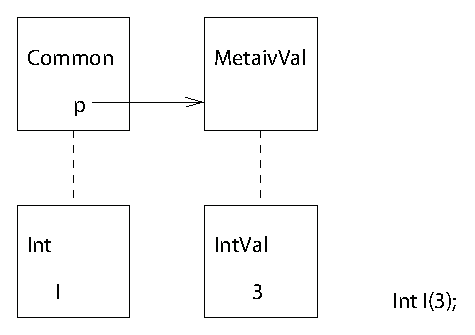
\includegraphics{fig1}}
%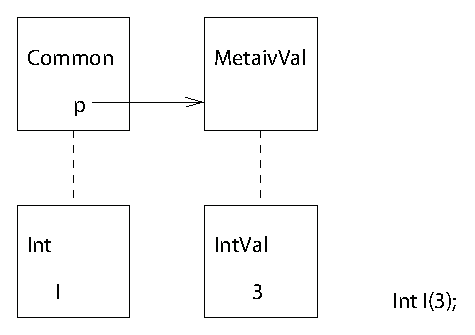
\includegraphics{fig1}
\caption{General structure.\label{fig1}}
\end{center}
\end{figure}

For all the VDM classes like {\tt Set}, {\tt Int}, {\tt Map}
etc.\ there exists a corresponding value class named {\tt SetVal},
{\tt IntVal}, {\tt MapVal} etc. All the VDM classes are
subclasses of the class {\tt Common}, whereas all the value classes
are subclasses of the class {\tt MetaivVal}.

When for instance a variable {\tt I} is declared of type {\tt Int},
instances of types {\tt Int} and {\tt IntVal} are created and a
pointer {\tt p} from the {\tt Int} instance (the pointer is actually
defined in {\tt Common}) is pointing to the {\tt IntVal} instance (it
is actually pointing to the {\tt MetaivVal} part of the {\tt IntVal}
instance). This situation is illustrated in Figure \ref{fig1}. The
dashed lines illustrate the class hierarchy and the solid line
illustrates the pointer {\tt p}. The value of {\tt I} is located in
the {\tt IntVal} instance. From now on when we refer to the value of a
variable we always mean the instance of the Val class which the
pointer {\tt p} points to.

\begin{figure}[hbt]
  \begin{center}
    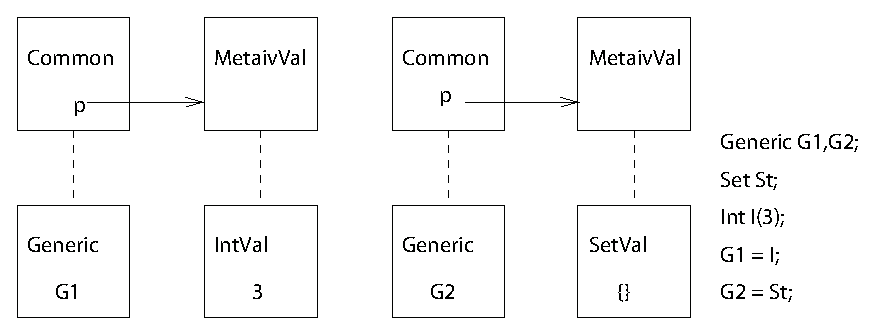
\includegraphics{fig2}
    \caption{Generics.\label{fig2}}
  \end{center}
\end{figure}


In order to support the idea of union types the {\tt Generic} class
has been introduced. This allows instances of the classes representing
compound VDM types ({\tt Map, Sequence, Tuple, Set, Record}) to
contain elements of different types at the same time. The value of a
generic can be any of the VDM values from the basics {\tt IntVal,
RealVal} to the compound values like {\tt TupleVal, SequenceVal}.
This means that a variable of type {\tt Generic} can have an
underlying value of any VDM type. Figure \ref{fig2} shows two
examples of generics.

In reality it is implemented such that the compound types only can
contain elements of type {\tt Generic} Most of the functions which
insert elements into compound types are able to automatically cast
elements to {\tt Generics} before inserting them, but functions which
retrieve elements will always return a {\tt Generic}.

To show an example of this let us look at the VDM expression:

\begin{verbatim}
let Sq = [1,<TWO>] in
  ...
\end{verbatim}

The sequence {\tt Sq} contains both an integer and a quote. As C++ is
strongly typed the C++ implementation of the let-expression must cast
the integer and the quote to {\tt Generic} before appending them to
the sequence {\tt Sq}. In the implementation below this casting is
done automatically by the {\tt ImpAppend} function, and the retrieve
function {\tt Hd()} returns a {\tt Generic}. As the first element in
the sequence is of type {\tt Int}, {\tt G} can later be cast to {\tt
Int}. 

\begin{verbatim}
Sequence Sq;  Generic G;

Sq.ImpAppend(Int(1)); 
Sq.ImpAppend(Quote(``<TWO>''));

G = Sq.Hd();
\end{verbatim}

In general, any type can be casted to a {\tt Generic}, but it will
only be generic on the surface and preserves the underlying value. For
instance, the generic {\tt G1} on Figure \ref{fig2} can later be
casted back to an {\tt Int}. For all the classes representing compound
types ({\tt Map, Sequence, Tuple, Set, Record}) all the elements
contained in the class will automatically be casted to {\tt Generic}
before they are included.  This means that when an element is
retrieved from a compound variable it will always be of type {\tt
  Generic}. It can then be casted back to the original type if
necessary.



\section{General functions on VDM types} 
\label{general-op}

This section describes all functions which are defined in class {\tt
Common} and therefore are applicable to instances of all types.
Note that {\tt true} in the following denotes an integer greater than
zero and {\tt false} denotes the integer value zero.

\subsection*{Functions}

\begin{description}
\item[{\tt A.MyValType()}] \mbox{}\\
     Returns the type of the value of {\tt A}.

     Result type : {\bf metaivType}
     
     \vspace{1cm}
     Note that the enumerate type {\tt metaivType} is a part of the
     library.

\begin{quote}
\begin{verbatim}
enum metaivType {
  mt_nil, mt_char, mt_int, mt_real, mt_quote,
  mt_tuple, mt_record, mt_set, mt_map, mt_generic,
  mt_text, mt_token, mt_bool, mt_sequence, 
  mt_objectref, mt_undef
}
\end{verbatim}
\end{quote}

\item[{\tt A1 = A2}] \mbox{}\\
     Gives {\tt A1} the value of {\tt A2}. If {\tt A1} is of type {\tt Generic}
     then {\tt A2} can be of any type. In that case {\tt A1} will
     still be a generic, but it will contain the value of {\tt A2}.
     Otherwise the type of the value
     of {\tt A2} must be the same as the type of the value of {\tt A1}.

     Result type : reference to A1. 
     
\item[{\tt A1 == A2}] \mbox{}\\
     Returns {\tt true} if the value of {\tt A1} equals the value
     of {\tt A2} and {\tt false} otherwise.

     Result type : {\bf bool}

\item[{\tt A1 != A2}] \mbox{}\\
     Returns {\tt true} if the value of {\tt A1} does not equal the value
     of {\tt A2} and {\tt false} otherwise.

     Result type : {\bf bool}

\item[{\tt A.ascii()}] \mbox{}\\
     Returns a {\tt wstring} containing an ASCII representation of the
     VDM value.

     Result type : {\bf wstring}
     
\item[{\tt A.IsNil()}] \mbox{}\\
     Returns {\tt true} if the value of {\tt A} is of type {\tt Nil}

     Result type : {\bf bool}
     
\item[{\tt A.IsChar()}] \mbox{}\\
     Returns {\tt true} if {\tt A} is of type {\tt Char}

     Result type : {\bf bool}

\item[{\tt A.IsInt()}] \mbox{}\\
     Returns {\tt true} if {\tt A} is of type {\tt Int}

     Result type : {\bf bool}

\item[{\tt A.IsReal()}] \mbox{}\\
     Returns {\tt true} if {\tt A} is of type {\tt Real}

     Result type : {\bf bool}

\item[{\tt A.IsQuote()}] \mbox{}\\
     Returns {\tt true} if {\tt A} is of type {\tt Quote}

     Result type : {\bf bool}

\item[{\tt A.IsTuple()}] \mbox{}\\
     Returns {\tt true} if {\tt A} is of type {\tt Tuple}

     Result type : {\bf bool}

\item[{\tt A.IsRecord()}] \mbox{}\\
     Returns {\tt true} if {\tt A} is of type {\tt Record}

     Result type : {\bf bool}

\item[{\tt A.IsSet()}] \mbox{}\\
     Returns {\tt true} if {\tt A} is of type {\tt Set}

     Result type : {\bf bool}

\item[{\tt A.IsMap()}] \mbox{}\\
     Returns {\tt true} if {\tt A} is of type {\tt Map}

     Result type : {\bf bool}

\item[{\tt A.IsText()}] \mbox{}\\
     Returns {\tt true} if {\tt A} is of type {\tt Text}

     Result type : {\bf bool}

\item[{\tt A.IsToken()}] \mbox{}\\
     Returns {\tt true} if {\tt A} is of type {\tt Token}

     Result type : {\bf bool}

\item[{\tt A.IsBool()}] \mbox{}\\
     Returns {\tt true} if {\tt A} is of type {\tt Bool}

     Result type : {\bf bool}

\item[{\tt A.IsSequence()}] \mbox{}\\
     Returns {\tt true} if {\tt A} is of type {\tt Sequence}

     Result type : {\bf bool}

\item[{\tt A.IsObjectRef()}] \mbox{}\\
     Returns {\tt true} if {\tt A} is of type {\tt ObjectRef}

     Result type : {\bf bool}


\item[{\tt A.WriteVal(o)}] \mbox{}\\
  Write the value of {\tt A} to the {\tt ostream} {\tt o}, in a format
  such that the value can be read in again using the function ReadVal.
  {\tt ReadVal} and {\tt WriteVal} is used for saving a value to the
  filesystem and later read it back (``persistency'').

  Return type: {\bf void}
  
\item[{\tt Generic g; g = ReadVal(i)}] \mbox{}\\
  Read in a value (through an istream) from a file that was written
  with the WriteVal method. Note that {\tt ReadVal} is a function, not
  a method.  
  
  The format that {\tt WriteVal} writes and {\tt ReadVal} reads is a
  low-level format not intended for humans.
  
  Return type: {\bf Generic}
\end{description}


\subsection*{Examples}

Example C++ program using the functions described in this section.

\begin{verbatim}
    Generic G1;  Int I1(3),I2(4),I3;

    G1 = I1;
    I3 = G1;
    if (G1 == I3)
      wcout << "The value of G1 equals the value of I3" << endl;
    if (G1.IsInt())
      wcout << "The value of G1 is of type Int" << endl;
      wcout << G1.MyValType() << "  The value of G1 is of type Int" << endl;
      wcout << I1.ascii()  << "  The ASCII representation of I1" << endl;
\end{verbatim}

\noindent The result of running this program is :

\begin{verbatim}
The value of G1 equals the value of I3
The value of G1 is of type Int
103  The value of G1 is of type Int
3  The ASCII representation of I1
\end{verbatim}

%\noindent Note that the values {\tt 2} corresponds to {\tt mt\_int}.

\subsection{Printing values to ostreams}
\label{sec:Printing}

Any VDM value \texttt{v} can be printed to an ostream \texttt{os} with
\texttt{os << v}. 

A Record will per default be printed with its numeric tag like this:
\path+mk_unknown4(...)+.
%insert
%�܂��A�^�O���𕶎��`���ň������ɂ́A\ref{The Record Information Map} The Record Information Map���g�p����B

\subsubsection*{Example}

\verbatimfile{tagmap.cc}

The result of running this program is :
\begin{verbatim}
r1=mk_X`a( 
mk_X`b( 
mk_X`b( 100 ) ) )
\end{verbatim}

\section{Specific functions on the VDM types} \label{specific-op}
\subsection{Int}
{\tt Int} supports the following member functions:

\vspace{0.5cm}

\begin{description}
\item[{\tt Int I}] \mbox{}\\
     Declares {\tt I} as an {\tt Int}. The value of {\tt I} is 
     initialized to 0. 

     Result type : {\bf void}
\item[{\tt Int I(i)}] \mbox{}\\
     Declares {\tt I} as an {\tt Int} and initializes the value to {\tt i}.

     Result type : {\bf void}

\item[{\tt Int I(I1)}] \mbox{}\\
     Declares {\tt I} as an {\tt Int} which is equal to {\tt I1}.

     Result type : {\bf void}

\item[{\tt I.GetValue()}] \mbox{}\\
     Returns the C++ integer value of {\tt I}.

     Result type : {\bf int}

\item[{\tt I = i}] \mbox{}\\
     Gives {\tt I} the value of {\tt i}.

     Result type : {\bf Int\&}

\item[{\tt -I}] \mbox{}\\
     Unary minus. Return an {\tt Int} with the negated value of {\tt I}.

     Result type : {\bf Int}

\item[{\tt I1 + I2}] \mbox{}\\
     Binary plus. 

     Result type : {\bf Int}

\item[{\tt I + R}] \mbox{}\\
     Binary plus. 

     Result type : {\bf Real}

\item[{\tt I1 - I2}] \mbox{}\\
     Binary minus. 

     Result type : {\bf Int}

\item[{\tt I - R}] \mbox{}\\
     Binary minus. 

     Result type : {\bf Real}

\item[{\tt I1 * I2}] \mbox{}\\
     Binary multiplication. 

     Result type : {\bf Int}

\item[{\tt I * R}] \mbox{}\\
     Binary multiplication. 

     Result type : {\bf Real}

\item[{\tt I1 / I2}] \mbox{}\\
     Binary division. 

     Division by zero causes an error cf.\ Section~\ref{error-messages}.

     Result type : {\bf Real}

\item[{\tt I / R}] \mbox{}\\
     Binary division. 

     Division by zero causes an error cf.\ Section~\ref{error-messages}.

     Result type : {\bf Real}

\item[{\tt I1.Exp(I2)}] \mbox{}\\
     Exponentiation. 

     Result type : {\bf Real}

\item[{\tt I.Exp(R)}] \mbox{}\\
     Exponentiation. 

     Result type : {\bf Real}

\end{description}

\subsection*{Examples}

\begin{verbatim}
    Int I1(3),I2;
    Int I3(I1);

    if (I1 == I3)
      wcout << "The value of I1 equals the value of I3" << endl;
      wcout << I2.GetValue() << "  is the initial value of I2" << endl;
    I2 = 10;
      wcout << I2.GetValue() << "  is the new value of I2" << endl;
\end{verbatim}

\noindent The result of running this program is :

\begin{verbatim}
The value of I1 equals the value of I3
0  is the initial value of I2
10  is the new value of I2
\end{verbatim}


\subsection{Real}
{\tt Real} supports the following member functions:

\vspace{0.5cm}

\begin{description}
\item[{\tt Real Rl}] \mbox{}\\
     Declares {\tt Rl} as a {\tt Real}. The value of {\tt Rl} is 
     initialized to 0. 

     Result type : {\bf void}

\item[{\tt Real Rl(d)}] \mbox{}\\
     Declares {\tt Rl} as a {\tt Real} and initializes the value to {\tt d}.

     Result type : {\bf void}

\item[{\tt Real Rl(Rl1)}] \mbox{}\\
     Declares {\tt Rl} as a {\tt Real} which is equal to {\tt Rl1}.

     Result type : {\bf void}

\item[{\tt Rl.GetValue()}] \mbox{}\\
     Returns the C++ double value of {\tt Rl}.

     Result type : {\bf double}
     
\item[{\tt Rl = d}] \mbox{}\\
     Gives {\tt Rl} the value of {\tt d}.

     Result type : {\bf Real\&}

\item[{\tt -R}] \mbox{}\\
     Unary minus. Returns a {\tt Real} with the negated value of {\tt R}.

     Result type : {\bf Real}

\item[{\tt R1 + R2}] \mbox{}\\
     Binary plus. 

     Result type : {\bf Real}

\item[{\tt R + I}] \mbox{}\\
     Binary plus. 

     Result type : {\bf Real}

\item[{\tt R1 - R2}] \mbox{}\\
     Binary minus. 

     Result type : {\bf Real}

\item[{\tt R - I}] \mbox{}\\
     Binary minus. 

     Result type : {\bf Real}

\item[{\tt R1 * R2}] \mbox{}\\
     Binary multiplication. 

     Result type : {\bf Real}

\item[{\tt R * I}] \mbox{}\\
     Binary multiplication. 

     Result type : {\bf Real}

\item[{\tt R1 / R2}] \mbox{}\\
     Binary division. 

     Result type : {\bf Real}

\item[{\tt R / I}] \mbox{}\\
     Binary division. 

     Result type : {\bf Real}

\item[{\tt R1.Exp(R2)}] \mbox{}\\
     Exponentiation. 

     Result type : {\bf Real}

\item[{\tt R.Exp(I)}] \mbox{}\\
     Exponentiation. 

     Result type : {\bf Real}
\end{description}

\subsection*{Examples}

\begin{verbatim}
    Real Rl1(3.2),Rl2;
    Real Rl3(Rl1);

    if (Rl1 == Rl3)
      wcout << "The value of Rl1 equals the value of Rl3" << endl;
      wcout << Rl2.GetValue() << "  is the initial value of Rl2" << endl;
    Rl2 = 10.5;
      wcout << Rl2.GetValue() << "  is the new value of Rl2" << endl;
\end{verbatim}

\noindent The result of running this program is :

\begin{verbatim}
The value of Rl1 equals the value of Rl3
0 is the initial value of Rl2
10.5  is the new value of Rl2
\end{verbatim}

\subsection{Bool}
{\tt Bool} supports the following member functions:

\vspace{0.5cm}

\begin{description}
\item[{\tt Bool B}] \mbox{}\\
     Declares {\tt B} as a {\tt Bool}. The value of {\tt B} is
     initialized to 0 ({\tt false}). 

     Result type : {\bf void}

\item[{\tt Bool B(i)}] \mbox{}\\
     Declares {\tt B} as a {\tt Bool} and initialize the value to {\tt i}.

     Result type : {\bf void}

\item[{\tt Bool B(B1)}] \mbox{}\\
     Declares {\tt B} as a {\tt Bool} which is equal to {\tt B1}.

     Result type : {\bf void}

\item[{\tt B.GetValue()}] \mbox{}\\
     Returns the C++ {\bf bool} of {\tt B}.

     Result type : {\bf bool}

\item[{\tt B = i}] \mbox{}\\
     Gives {\tt B} the value of {\tt i}.

     Result type : {\bf Bool\&}

\item[{\tt B.not()}] \mbox{}\\
     Logical negation.

     Result type : {\bf Bool}

\item[{\tt !B}] \mbox{}\\
     Logical negation.

     Result type : {\bf Bool}

\item[{\tt B1.and(B2)}] \mbox{}\\
     Logical and.

     Result type : {\bf Bool}

\item[{\tt B1 \&\& B2}] \mbox{}\\
     Logical and.

     Result type : {\bf Bool}

\item[{\tt B1.or(B2)}] \mbox{}\\
     Logical or.

     Result type : {\bf Bool}

\item[{\tt B1 || B2}] \mbox{}\\
     Logical or.

     Result type : {\bf Bool}

\end{description}

\subsection*{Examples}

\begin{verbatim}
    Bool B1(3),B2;
    Bool B3(B1);

    if (B1 == B3)
      wcout << "The value of B1 equals the value of B3" << endl;
      wcout << B2.GetValue() << "  is the initial value of B2" << endl;
    B2 = 1;
      wcout << B2.GetValue() << "  is the new value of B2 (true)" << endl;
\end{verbatim}

\noindent The result of running this program is :

\begin{verbatim}
    The value of B1 equals the value of B3
    0  is the initial value of B2
    1  is the new value of B2 (true)
\end{verbatim}


\subsection{Nil}
{\tt Nil} support the following member functions:

\vspace{0.5cm}

\begin{description}
\item[{\tt Nil N}] \mbox{}\\
     Declares {\tt N} as a value of type {\tt Nil}.

     Result type : {\bf void}

\end{description}

\noindent Instances of type {\tt Nil} only support the functions which
are common to all types (see section \ref{general-op}).


\subsection{Quote}
{\tt Quote} supports the following member functions:

\vspace{0.5cm}

\begin{description}
\item[{\tt Quote Q}] \mbox{}\\
     Declares {\tt Q} as a value of type {\tt Quote}. The value of {\tt Q}
     is initialized to {\tt ""}.

     Result type : {\bf void}

\item[{\tt Quote Q(s)}] \mbox{}\\
     Declares {\tt Q} as a value of type {\tt Quote} and initialize
     the value to {\tt s}.

     Result type : {\bf void}

\item[{\tt Quote Q(Q1)}] \mbox{}\\
     Declares {\tt Q} as a value of type {\tt Quote} which is equal to
     {\tt Q1}.

     Result type : {\bf void}

\item[{\tt Q.GetValue()}] \mbox{}\\
     Returns the C++ wstring value of {\tt Q}.

     Result type : {\bf wstring}

\item[{\tt Q = s}] \mbox{}\\
     Gives {\tt Q} the value of {\tt s}.

     Result type : {\bf Quote\&}
\end{description}

\subsection*{Examples}

\begin{verbatim}
    Quote Q1("Q_ONE"),Q2;
    Quote Q3(Q1);

    if (Q1 == Q3)
      wcout << "The value of Q1 equals the value of Q3" << endl;
      wcout << Q2.GetValue() << "  is the initial value of Q2" << endl;
    Q2 = "Q_TWO";
      wcout << Q2.GetValue() << "  is the new value of Q2" << endl;
\end{verbatim}

\noindent The result of running this program is :

\begin{verbatim}
    The value of Q1 equals the value of Q3
      is the initial value of Q2
    Q_TWO  is the new value of Q2
\end{verbatim}


\subsection{Char}
{\tt Char} supports the following member functions:

\vspace{0.5cm}

\begin{description}
\item[{\tt Char C}] \mbox{}\\
     Declares {\tt C} as a value of type {\tt Char}. The value of {\tt C}
     is initialized to {\tt '?'}.

     Result type : {\bf void}

\item[{\tt Char C(c)}] \mbox{}\\
     Declares {\tt C} as a value of type {\tt Char} and initializes
     the value to {\tt c}.

     Result type : {\bf void}

\item[{\tt Char C(C1)}] \mbox{}\\
     Declares {\tt C} as a value of type {\tt Char} which is equal to
     {\tt C1}.

     Result type : {\bf void}

\item[{\tt C.GetValue()}] \mbox{}\\
     Returns the C++ wchar\_t value of {\tt C}.

     Result type : {\bf wchar\_t}
     
\item[{\tt C = c}] \mbox{}\\
     Gives {\tt C} the value of {\tt c}.

     Result type : {\bf Char\&}
\end{description}

\subsection*{Examples}

\begin{verbatim}
    Char C1('c'),C2;
    Char C3(C1);

    if (C1 == C3)
      wcout << "The value of C1 equals the value of C3" << endl;
      wcout << C2.GetValue() << "  is the initial value of C2" endl;
    C2 = 'd';
      wcout << C2.GetValue() << "  is the new value of C2" << endl;
\end{verbatim}

\noindent The result of running this program is :

\begin{verbatim}
    The value of C1 equals the value of C3
    ?  is the initial value of C2
    d  is the new value of C2
\end{verbatim}


\subsection{Text}
{\tt Text} supports the following member functions:

\vspace{0.5cm}

\begin{description}
\item[{\tt Text Tx}] \mbox{}\\
     Declares {\tt Tx} as a value of type {\tt Text}. The value of {\tt Tx}
     is initialized to {\tt ""}.

     Result type : {\bf void}

\item[{\tt Text Tx(s)}] \mbox{}\\
     Declares {\tt Tx} as a value of type {\tt Text} and initializes
     the value to {\tt s}.

     Result type : {\bf void}

\item[{\tt Text Tx(Tx1)}] \mbox{}\\
     Declares {\tt Tx} as a value of type {\tt Text} which is equal to
     {\tt Tx1}.

     Result type : {\bf void}

\item[{\tt Tx.GetValue()}] \mbox{}\\
     Returns the C++ wstring value of {\tt Tx}.

     Result type : {\bf wstring}

\item[{\tt Tx = s}] \mbox{}\\
     Gives {\tt Tx} the value of {\tt s}.

     Result type : {\bf Text\&}
\end{description}

\subsection*{Examples}

\begin{verbatim}
    Text Tx1("Tx_ONE"),Tx2;
    Text Tx3(Tx1);

    if (Tx1 == Tx3)
      wcout << "The value of Tx1 equals the value of Tx3" << endl;
      wcout << Tx2.GetValue() << "  is the initial value of Tx2" <<endl;
    Tx2 = "Tx_TWO";
      wcout << Tx2.GetValue() << "  is the new value of Tx2" << endl;
\end{verbatim}

\noindent The result of running this program is :

\begin{verbatim}
    The value of Tx1 equals the value of Tx3
      is the initial value of Tx2
    Tx_TWO  is the new value of Tx2
\end{verbatim}


\subsection{Token}
{\tt Token} supports the following member functions:

\vspace{0.5cm}

\begin{description}
\item[{\tt Token Tk}] \mbox{}\\
     Declares {\tt Tk} as a value of type {\tt Token}. The value of {\tt Tk}
     is initialized to {\tt ""}.

     Result type : {\bf void}

\item[{\tt Token Tk(s)}] \mbox{}\\
     Declares {\tt Tk} as a value of type {\tt Token} and initializes
     the value to {\tt s}.

     Result type : {\bf void}

\item[{\tt Token Tk(Tk1)}] \mbox{}\\
     Declares {\tt Tk} as a value of type {\tt Token} which is equal to
     {\tt Tk1}.

     Result type : {\bf void}

\item[{\tt Tk.GetValue()}] \mbox{}\\
     Returns the C++ wstring value of {\tt Tk}.

     Result type : {\bf wstring}

\item[{\tt Tk = s}] \mbox{}\\
     Gives {\tt Tk} the value of {\tt s}.

     Result type : {\bf Token\&}
\end{description}

\subsection*{Examples}

\begin{verbatim}
    Token Tk1("Tk_ONE"),Tk2;
    Token Tk3(Tk1);

    if (Tk1 == Tk3)
      wcout << "The value of Tk1 equals the value of Tk3" << endl;
      wcout << Tk2.GetValue() << "  is the initial value of Tk2" << endl;
    Tk2 = "Tk_TWO";
      wcout << Tk2.GetValue() << "  is the new value of Tk2" <<endl;
\end{verbatim}

\noindent The result of running this program is :

\begin{verbatim}
    The value of Tk1 equals the value of Tk3
      is the initial value of Tk2
    Tk_TWO  is the new value of Tk2
\end{verbatim}




\subsection{Map}
{\tt Map} supports the following member functions:

\vspace{0.5cm}

\begin{description}
\item[{\tt Map M}] \mbox{}\\
     Declares {\tt M} as a value of type {\tt Map} and initializes it
     to the empty map.

     Result type : {\bf void}

\item[{\tt Map M(M1)}] \mbox{}\\
     Declares {\tt M} as a value of type {\tt Map} and initializes it to
     {\tt M1}.

     Result type : {\bf void}

\item[{\tt M.Insert(A1, A2)}] \mbox{}\\
     Inserts the key {\tt A1} with the associated contents {\tt A2}
     in {\tt M}. If the key {\tt A1} already belongs to the domain of
     {\tt M} it is checked whether A2 is equal to the range value. 
     If not, then an error is signaled cf.\ Section~\ref{error-messages}. 
     The function returns a reference to {\tt M}.

     Result type : {\bf Map\&}

\item[{\tt M.ImpModify(A1, A2)}] \mbox{}\\
     Works as {\tt Insert} except that if the key {\tt A1} already
     belongs to the domain of {\tt M} the range value is modified
     to {\tt A2}. The function returns a reference to {\tt M}. 

     Result type : {\bf Map\&}
 
\item[{\tt M[A]}] \mbox{}\\
     Returns the contents associated with the key {\tt A}. If {\tt A}
     is not in the domain for {\tt M} an error is signaled cf.\ 
     Section~\ref{error-messages}. 

     Result type : {\bf Generic\&}

\item[{\tt M.ImpOverride(M1)}] \mbox{}\\     
     {\tt M} becomes the union of {\tt M} and {\tt M1}. If a key in
     {\tt M} also exists in {\tt M1} the corresponding contents in {\tt M}
     is overriden by the contents in {\tt M1}. 
     The function returns a reference to {\tt M}.

     Result type : {\bf Map\&}

\item[{\tt M.Size()}] \mbox{}\\
     Returns an integer denoting the number of keys in {\tt M}.

     Result type : {\bf int}

\item[{\tt M.IsEmpty()}] \mbox{}\\
     Returns {\tt true} if {\tt M.Size() == 0} and {\tt false} otherwise.

     Result type : {\bf bool}
     
\item[{\tt M.Dom()}] \mbox{}\\     
     Returns a Set containing all the keys in {\tt M}.    

     Result type : {\bf Set}
     
\item[{\tt M.Rng()}] \mbox{}\\     
     Returns a Set containing all the contents in {\tt M}.    

     Result type : {\bf Set}

\item[{\tt M.DomExists(A)}] \mbox{}\\     
     Returns {\tt true} if {\tt A} is in the domain of {\tt M} and {\tt false} otherwise.

     Result type : {\bf bool}

\item[{\tt M.RemElem(A)}] \mbox{}\\     
     If {\tt A} is in the domain of {\tt M} remove both key and
     contents element, otherwise an error is signaled
     cf.\ Section~\ref{error-messages}. 

     Result type : {\bf Map\&}

\item[{\tt M.First(G)}] \mbox{}\\     
     Returns 1 if {\tt M} is not empty and returns the first key in
     the reference parameter {\tt G}, according to an internal
     ordering. If {\tt M} is empty it returns 0
     and G will be returned as an empty Generic.

     Result type : {\bf bool}
     
\item[{\tt M.Next(G)}] \mbox{}\\
     Returns 1 and the next key in
     the reference parameter {\tt G}. If there are no more keys in {\tt M}
     it returns 0 and G will be returned as an empty Generic.

     Result type : {\bf bool}
\end{description}

\subsection*{Examples}

\begin{verbatim}
    Map M1,M2;  Set St;  Int I(5);  Generic G;

    M1.Insert(I,St).Insert(Int(7),St);
    M2.Insert(I,Int(1));
      wcout << M1.ascii() << " is the value of M1 before overriding" << endl;
    M1.ImpOverride(M2);        
      wcout << M1.ascii() << " is the value of M1 after overriding" << endl; 
      wcout << M1.Size() << " is the size of M1" << endl;
      wcout << M1.Dom().ascii() << " is the domain of M1" << endl;
    
    for (int b = M1.First(G); b; b = M1.Next(G))
      wcout << G.ascii() << " is a key of M1" << endl;
\end{verbatim}

\noindent The result of running this program is :

\begin{verbatim}
    { 5 |-> {  }, 7 |-> {  } } is the value of M1 before overriding
    { 5 |-> 1, 7 |-> {  } } is the value of M1 after overriding
    2 is the size of M1
    { 5, 7 } is the domain of M1
    5 is a key of M1
    7 is a key of M1
\end{verbatim}



\subsection{Sequence}

Elements in a {\tt Sequence} are indexed from 1 to the length of the
sequence. {\tt Sequence} supports the following member functions:

\vspace{0.5cm}

\begin{description}
\item[{\tt Sequence Sq}] \mbox{}\\
     Declares {\tt Sq} as a value of type {\tt Sequence} and
     initializes it to the empty sequence.

     Result type : {\bf void}

\item[{\tt Sequence Sq(Sq1)}] \mbox{}\\
     Declares {\tt Sq} as a value of type {\tt Sequence} and
     initializes it to {\tt Sq1}.

     Result type : {\bf void}

\item[{\tt Sequence Sq(s)}] \mbox{}\\
     Declares {\tt Sq} as a value of type {\tt Sequence} and
     initializes it to the  {\tt wstring} {\tt s} converted to a 
     ``{\tt seq of char}''.

     Result type : {\bf void}

\item[{\tt Sq[i]}] \mbox{}\\     
     Returns the {\tt i}'th element in {\tt Sq}. If {\tt i} is not
     a valid index, an error is signaled
     cf. Section~\ref{error-messages}.  

     Result type : {\bf Generic\&}

\item[{\tt Sq.Index(i)}] \mbox{}\\     
     Returns the {\tt i}'th element in {\tt Sq}. If {\tt i} is not
     a valid index, an error is signaled
     cf. Section~\ref{error-messages}.

     Result type : {\bf Generic\&}

\item[{\tt Sq.Hd()}] \mbox{}\\     
     Returns the first element in {\tt Sq}. If {\tt Sq} is the empty
     sequence, an error is signaled cf. Section~\ref{error-messages}.

     Result type : {\bf Generic\&}

\item[{\tt Sq.Tl()}] \mbox{}\\     
     Returns the tail of {\tt Sq}. If {\tt Sq} is the empty
     sequence, an error is signaled cf. Section~\ref{error-messages}.

     Result type : {\bf Sequence}

\item[{\tt Sq.ImpTl()}] \mbox{}\\     
     Changes {\tt Sq} to the tail of {\tt Sq}. If {\tt Sq} is the empty
     sequence, an error is signaled cf. Section~\ref{error-messages}.

     The function returns a reference to {\tt Sq}. 

     Result type : {\bf Sequence\&}

\item[{\tt Sq.RemElem(int i)}] \mbox{}\\
     Removed the {\tt i}'th element from {\tt Sq} given that {\tt i} is a
     valid index for {\tt Sq}. If it is not, an error is signaled
     cf. Section~\ref{error-messages}.

     The function returns a reference to {\tt Sq}.

     Result type: {\bf Sequence\&}

\item[{\tt Sq.Length()}] \mbox{}\\     
     Returns an integer denoting the number of elements in {\tt Sq}.

     Result type : {\bf int}

\item[{\tt Sq.GetString(string\& str)}] \mbox{}\\     
  Convert a ``{\tt seq of char}'' to {\tt wstring}.  

  Returns {\tt true} if all elements in {\tt Sq} is of type Char and
  the string representation of {\tt Sq} in the parameter {\tt str}.
  Otherwise {\tt GetString} will return {\tt false} and set {\tt str}
  to the empty string ({\tt ""}).
  
  Result type : {\bf bool}

\item[{\tt Sq.IsEmpty()}] \mbox{}\\     
     Returns 0 if {\tt Sq} is empty and 1 otherwise.

     Result type : {\bf bool}

\item[{\tt Sq.ImpAppend(A)}] \mbox{}\\     
     Appends {\tt A} to {\tt Sq} and places the result in {\tt Sq}.
     The function returns a reference to {\tt Sq}.

     Result type : {\bf Sequence\&}

\item[{\tt Sq.ImpModify(i,A)}] \mbox{}\\     
     Modifies the {\tt i}'th element in {\tt Sq} to {\tt A}. If {\tt i} is not
     a valid index an error is signaled cf. Section~\ref{error-messages}.
     The function returns a reference to {\tt Sq}.

     Result type : {\bf Sequence\&}

\item[{\tt Sq.ImpPrepend(A)}] \mbox{}\\     
     Prepends {\tt A} to {\tt Sq} and places the result in {\tt Sq}.
     The function returns a reference to {\tt Sq}.

     Result type : {\bf Sequence\&}

\item[{\tt Sq.ImpConc(Sq1)}] \mbox{}\\     
     Concatenates {\tt Sq} and {\tt Sq1} and places the result in {\tt Sq}.
     The function returns a reference to {\tt Sq}.

     Result type : {\bf Sequence\&}

\item[{\tt Sq.Elems()}] \mbox{}\\     
     Constructs a {\tt Set} containing all elements in {\tt Sq}. The
     {\tt Set} is returned.

     Result type : {\bf Set}

\item[{\tt Sq.First(G)}] \mbox{}\\     
     Returns 1 if {\tt Sq} is not empty and returns the first element in
     the reference parameter {\tt G}. If {\tt Sq} is empty it returns 0
     and G will be returned as an empty Generic.

     Result type : {\bf bool}
     
\item[{\tt Sq.Next(G)}] \mbox{}\\     
     Returns 1 and the next element in
     the reference parameter {\tt G}. If there are no more keys in {\tt Sq}
     it returns 0 and G will be returned as an empty Generic.

     Result type : {\bf bool}
\end{description}

\subsection*{Examples}

\begin{verbatim}
    Sequence Sq1,Sq2;  Set St;  Int I(5);  Generic G;

    if (Sq1.IsEmpty()) 
      wcout << "Sq1 is initialized to the empty sequence" << endl;
      wcout << Sq1.ImpAppend(I).ImpPrepend(St).Length()
         << " is the length of Sq1" << endl;
      wcout << Sq1.ImpTl().ascii()
         << " is the value of Sq1 after applying ImpTl" << endl;
    Sq2.ImpAppend(Sq1.Hd());
      wcout << Sq1.ImpConc(Sq2).Length()
         << " is the length of Sq1 after applying ImpConc" << endl;
\end{verbatim}

\noindent The result of running this program is :

\begin{verbatim}
    Sq1 is initialized to the empty sequence
    2 is the length of Sq1
    [ 5 ] is the value of Sq1 after applying ImpTl
    2 is the length of Sq1 after applying ImpConc
\end{verbatim}



\subsection{Set}
{\tt Set} supports the following member functions:

\vspace{0.5cm}

\begin{description}
\item[{\tt Set St}] \mbox{}\\
     Declares {\tt St} as a value of type {\tt Set} and
     initializes it to the empty set.

     Result type : {\bf void}

\item[{\tt Set St(St1)}] \mbox{}\\
     Declares {\tt St} as a value of type {\tt Set} which is equal to
     {\tt St1}.

     Result type : {\bf void}

\item[{\tt St.Insert(A)}] \mbox{}\\     
     Inserts {\tt A} in {\tt St}. If {\tt A} already exists in {\tt
     St}, {\tt St} is left unchanged.
     The function returns a reference to {\tt St}.

     Result type : {\bf Set\&}

\item[{\tt St.Card()}] \mbox{}\\     
     Returns an integer denoting the number of elements in {\tt St}.

     Result type : {\bf int}

\item[{\tt St.IsEmpty()}] \mbox{}\\
     Returns {\tt true} if {\tt St.Card() == 0} and {\tt false} otherwise.

     Result type : {\bf bool}
     
\item[{\tt St.InSet(A)}] \mbox{}\\     
     Returns 1 if {\tt A} is in {\tt St} and 0 otherwise.

     Result type : {\bf bool}

\item[{\tt St.ImpUnion(St1)}] \mbox{}\\     
     Adds all elements of {\tt St1} to {\tt St}.
     The function returns a reference to {\tt St}.

     Result type : {\bf Set\&}

\item[{\tt St.ImpIntersect(St1)}] \mbox{}\\     
     Removes all elements of {\tt St} not occuring in {\tt St1}.
     The function returns a reference to {\tt St}.

     Result type : {\bf Set\&}

\item[{\tt St.GetElem()}] \mbox{}\\     
     Returns an element {\tt G} from {\tt St}. If {\tt St} is empty an
     error is signaled cf.\ Section~\ref{error-messages}.

     Result type : {\bf Generic\&}

\item[{\tt St.RemElem(A)}] \mbox{}\\     
     Removes {\tt A} from {\tt St}. If {\tt A} is not in {\tt St} an
     error is signaled cf.\ Section~\ref{error-messages}. 
     The function returns a reference to {\tt St}.

     Result type : {\bf Set\&}

\item[{\tt St.SubSet(St1)}] \mbox{}\\     
     Returns 1 if {\tt St} is a subset of {\tt St1} and 0 otherwise.

     Result type : {\bf bool}

\item[{\tt St.ImpDiff(St1)}] \mbox{}\\     
     Removes all elements of {\tt St1} from {\tt St}.
     The function returns a reference to {\tt St}.

     Result type : {\bf Set\&}

\item[{\tt St.First(G)}] \mbox{}\\     
     Returns 1 if {\tt St} is not empty and returns the first element in
     the reference parameter {\tt G}. If {\tt St} is empty it returns 0
     and G will be returned as an empty Generic.

     Result type : {\bf bool}
     
\item[{\tt St.Next(G)}] \mbox{}\\     
     Returns 1 and the next element in
     the reference parameter {\tt G}. If {\tt St} is empty
     it returns 0 and G will be returned as an empty Generic.

     Result type : {\bf bool}
\end{description}

\subsection*{Examples}
\begin{verbatim}
    Set St1,St2;  Int I(5);  Generic G;

    St1.Insert(I).Insert(St2);
    if (St1.InSet(I))
      wcout << "St1 contains I" << endl;
    St2.Insert(I).Insert(St1);
      wcout << St1.ImpUnion(St2).ascii() 
         << " is the union of St1 and St2" << endl;   
      wcout << St1.ImpIntersect(St2).ascii() 
         << " is the intersection of St1 and St2" << endl;   
\end{verbatim}

\noindent The result of running this program is :

\begin{verbatim}
    St1 contains I
    { 5, {  }, { 5, {  } } } is the union of St1 and St2
    { 5, { 5, {  } } } is the intersection of St1 and St2
\end{verbatim}

\subsection{Record}
{\tt Record} supports the following member functions:

\vspace{0.5cm}

\begin{description}
\item[{\tt Record Rc}] \mbox{}\\
     Declares {\tt Rc} as a value of type {\tt Record}. The number of
     fields is set to 0, and the tag is set to 0.

     Result type : {\bf void}

\item[{\tt Record Rc(i1,i2)}] \mbox{}\\
     Declares {\tt Rc} as a value of type {\tt Record} with the tag
     {\tt i1} and {\tt i2} fields. Note that the tag value -1 is
     reserved and must therefore not be used.

     Result type : {\bf void}

\item[{\tt Record Rc(Rc1)}] \mbox{}\\
     Declares {\tt Rc} as a value of type {\tt Record} which is equal to
     {\tt Rc1}.

     Result type : {\bf void}

\item[{\tt Rc.SetField(i,A)}] \mbox{}\\
     Modifies the {\tt i}'th field to {\tt A}. If {\tt i} is not
     within the defined number of fields for {\tt Rc} an error is
     signaled cf.\ Section~\ref{error-messages}. 
     The function returns a reference to {\tt Rc}.

     Result type : {\bf Record\&}

\item[{\tt Rc.GetField(i)}] \mbox{}\\
     Returns the contents {\tt G} of the {\tt i}'th field of {\tt Rc}.
     If {\tt i} is not within the range of the defined number of fields for
     {\tt Rc} an error is signaled cf.\  Section~\ref{error-messages}.     

     Result type : {\bf Generic\&}

\item[{\tt Rc.GetTag()}] \mbox{}\\
     Returns the tag {\tt i} of {\tt Rc}.

     Result type : {\bf int}

\item[{\tt Rc.Is(i)}] \mbox{}\\
     Returns 1 if {\tt i} equals the tag of {\tt Rc} and 0 otherwise.

     Result type : {\bf bool}

\item[{\tt Rc.Length()}] \mbox{}\\
     Returns the number of fields declared for {\tt Rc}.

     Result type : {\bf int}

\end{description}

\subsection*{Examples}

\begin{verbatim}
    #define Ex 1
    
    Record Rc1(Ex,2);  Int I(5);  Set St;

    Rc1.SetField(1,I).SetField(2,St);
    if (Rc1.Is(Ex))
      wcout << Rc1.GetTag() << " is the tag of Rc1" << endl;    
      wcout << Rc1.GetField(1).ascii() 
         << " is the value of the first field of Rc1" << endl;
      wcout << Rc1.Length() << " is the number of fields in Rc1" << endl;
\end{verbatim}

\noindent The result of running this program is :

\begin{verbatim}
    1 is the tag of Rc1
    5 is the value of the first field of Rc1
    2 is the number of fields in Rc1
\end{verbatim}


\subsubsection{The Record Information Map}

It is not legal to define a record with the same tag with different
size in the VDM Library. The VDM Library provides an internal state in
which it is possible to define relations between tag, size and string
tag of a record. The default internal st
ate can be accessed through
the function {\em VDMGetDefaultRecInfoMap}. The state and its member
functions is defined in class {\em VDMRecInfoMap} that supports the
following public member functions:

\begin{description}
\item[{\tt VDMRecInfoMap ri}]\mbox{}\\
  Declares {\tt ri} as a value of type {\tt VDMRecInfoMap}.

  Result type : {\bf void}
\item[{\tt NewTag(int tag, int size)}] \mbox{}\\
  Declares a new tag and size.

  Result type : {\bf void}
\item[{\tt AskDontCare(int tag, int size, int field)  }] \mbox{}\\
  
  Returns {\tt true} if field number {\em field} of the record
  declared with tag {\em tag} is an abstract field select.

  Result type : {\bf bool}

\item[{\tt AskDontCare(int tag, int field)  }] \mbox{}\\
  
  Returns {\tt true} if field number {\em field} of the record
  declared with tag {\em tag} is an abstract field select.

  Result type : {\bf bool}

\item[{\tt SetDontCare(int tag, int size, int field)}]\mbox{}\\

  Mark field number {\tt field} as an abstract field select for the
  record with tag number {\em tag}.

  Result type : {\bf void}

\item[{\tt SetDontCare(int tag, int field)}]\mbox{}\\

  Mark field number {\tt field} as an abstract field select for the
  record with tag number {\em tag}.

  Result type : {\bf void}

\item[{\tt SetSymTag(int tag, int size, const wstring\& symtag)}]\mbox{}\\
  
  Set the symbolic tag (the string tag of the record) of tag number
  {\em tag} to {\em symtag}. 
  This will relate {\em tag} to {\em symtab} in the {\em
  VDMRecInfoMap}. When using the {\em ascii} method for printing out
  record values and if a symbolic tag has been defined for a specific
  tag number, the symbolic tag string will be printed instead of the
  tag number {\em tag}.

  Result type : {\bf void}

\item[{\tt SetSymTag(int tag,  const wstring\& symtag)}]\mbox{}\\

  Set the symbolic tag (the string tag of the record) of tag number
  {\em tag} to {\em symtag}. 
  This will relate {\em tag} to {\em symtab} in the {\em
  VDMRecInfoMap}. When using the {\em ascii} method for printing out
  record values and if a symbolic tag has been defined for a specific
  tag number, the symbolic tag string will be printed instead of the
  tag number {\em tag}.

  Result type : {\bf void}

\item[{\tt SetPrintFunction(int tag, int size,
    vdm\_pp\_function\_ptr f)}]  \mbox{}\\
  
  With this function it is possible to relate a pointer to a function
  {\em f} to tag number {\em tag}. The function {\em f} will be used
  when calling the {\em ascii} method on the record with the tag {\em
  tag}.

  Result type : {\bf void}

\item[{\tt SetPrintFunction(int tag, int size, vdm\_pp\_function\_ptr f)}]  \mbox{}\\
  
  With this function it is possible to relate a pointer to a function
  {\em f} to tag number {\em tag}. The function {\em f} will be used
  when calling the {\em ascii} method on the record with the tag {\em
  tag}.

  Result type : {\bf void}

\item[{\tt GetSize(int tag)}]  \mbox{}\\

  Returns the size of the record that was declared with tag number
  {\em tag}.

  Result type : {\bf int}

%\item[{\tt GetSymTag(int tag, int size, wstring \& s)}]  \mbox{}\\
%
%  Extracts the symbolic string tag and assigns it to string {\em s} of
%  the record {\em tag}.
%
%  Result type : {\bf bool}

\item[{\tt GetSymTag(int tag, wstring \& s)}]  \mbox{}\\

  Extracts the symbolic string tag and assigns it to wstring {\em s} of
  the record {\em tag}.

  Result type : {\bf bool}


\item[{\tt size()}]  \mbox{}\\

  Returns the size of the map {\em VDMRecInfoMap}.

  Result type : {\bf int}

\item[{\tt dump(ostream \& o}]  \mbox{}\\

  Prints the information in the {\em VDMRecInfoMap} to the ostream
  {\em o}.

  Result type : {\bf void}

\end{description}


\subsection{Tuple}
{\tt Tuple} supports the following member functions:

\vspace{0.5cm}

\begin{description}
\item[{\tt Tuple Tp}] \mbox{}\\
     Declares {\tt Tp} as a value of type {\tt Tuple}. The number of
     fields is set to 0.

     Result type : {\bf void}

\item[{\tt Tuple Tp(i)}] \mbox{}\\
     Declares {\tt Tp} as a value of type {\tt Tuple} with {\tt i}
     fields.

     Result type : {\bf void}

\item[{\tt Tuple Tp(Tp1)}] \mbox{}\\
     Declares {\tt Tp} as a value of type {\tt Tuple} which is equal to
     {\tt Tp1}.

     Result type : {\bf void}

\item[{\tt Tp.SetField(i,A)}] \mbox{}\\
     Modifies the {\tt i}'th field to {\tt A}. If {\tt i} is not
     within the defined number of fields for {\tt Tp} an error is
     signaled cf.\ Section~\ref{error-messages}.
     The function returns a reference to {\tt Tp}.

     Result type : {\bf Tuple\&}

\item[{\tt Tp.GetField(i)}] \mbox{}\\
     Returns the contents {\tt G} of the {\tt i}'th field of {\tt Tp}.
     If {\tt i} is not within the defined number of fields for {\tt
     Tp} an error is
     signaled cf.\ Section~\ref{error-messages}.

     Result type : {\bf Generic\&}

\item[{\tt Tp.Length()}] \mbox{}\\
     Returns the number of fields declared for {\tt Tp}.

     Result type : {\bf int}
\end{description}

\subsection*{Examples}

\begin{verbatim}
    Tuple Tp1(2);  Int I(5);  Set St;

    Tp1.SetField(1,I).SetField(2,St);
      wcout << Tp1.GetField(1).ascii() 
         << " is the value of the first field of Tp1" << endl;
      wcout << Tp1.Length() << " is the number of fields in Tp1" << endl;
\end{verbatim}


\noindent The result of running this program is :

\begin{verbatim}
    5 is the value of the first field of Tp1
    2 is the number of fields in Rc1
\end{verbatim}

\subsection{ObjectRef}

The class ObjectRef is used to implement the object reference type in
VDM$^{++}$ \cite{AFROCGEDLRM}. This class should only be used to
contain references to instances of classes generated by the {\it VDM++
  to C++ Code Generator} \cite{CGManPP-CSK}.

ObjectRef contains a reference (pointer) to an instance of a C++
class, and a type variable identifying the type of the instance
pointed to by the refernce pointer. 

As the implementation of the VDM C++ library is based on reference
counters, it will delete the pointer to the instance of a class when
no existing objects of class \texttt{ObjectRef} refer to it. 

%The user must define a clean-up function {\tt DeleteUserClass} which
%the garbage collector uses. The signature for this function is defined
%in {\tt metaiv.h} (see appendix \ref{files}) and looks like:

%\begin{verbatim}
%void DeleteUserClass (void* p, int ct);
%\end{verbatim}

%The destructor for a {\tt ClassVal} will always call this function with
%the reference pointer and the type (see example).

{\tt ObjectRef} supports the following member functions:

\vspace{0.5cm}

\begin{description}
\item[{\tt ObjectRef Ob (p)}] \mbox{}\\
     Declares {\tt Ob} as a value of type {\tt ObjectRef}. The reference
     pointer is set to {\tt p}.
     A reference pointer must have been created with the C++ {\tt new}
     operator, in order for the built-in garbage collector to work
     correctly. The {\tt NULL} pointer will be used as default
     parameter, if no pointer is specified. 
     
     Result type : {\bf void}

\item[{\tt ObjectRef Ob(Ob1)}] \mbox{}\\
     Declares {\tt Ob} as a value of type {\tt ObjectRef} which is equal to
     {\tt Ob1}.

     Result type : {\bf void}

\item[{\tt Ob.MyObjectId()}] \mbox{}\\
     Returns the type {\tt i} of {\tt Ob}. The type is an integer
     defined as an enumeration type in \texttt{CGBase.h}

     Result type : {\bf int}

\item[{\tt Ob.GetRef()}] \mbox{}\\
     Returns the vdmBase pointer {\tt p} of {\tt Ob}.

     Result type : {\bf vdmBase*}

\item[\texttt{Ob.SameBaseClass(Ob1)}] \mbox{}\\
     Returns \texttt{True} if \texttt{Ob} and \texttt{Ob1} 
     has same base class, i.e. if \texttt{Ob} and \texttt{Ob1} are
     instances of classes that can be derived from the same root
     superclass, and \texttt{False} otherwise. 

     Result type : \textbf{Bool}
     
\item[\texttt{Ob.IsOfClass(i)}] \mbox{}\\
     Returns \texttt{True} if \texttt{Ob} refers to an object of a class
     with type \texttt{i} or any subclasses of \texttt{i}, and
     \texttt{False} otherwise. \texttt{i}
     is the type returned by \texttt{MyObjectId}.

     Result type : \textbf{Bool}

\item[\texttt{Ob.IsOfBaseClass(i)}] \mbox{}\\
     Returns \texttt{True} if the class with type \texttt{i} is a
     root  superclass in the inheritance chain of the object
     referenced to by \texttt{Ob}, and \texttt{False} otherwise.

     Result type : \textbf{Bool}

\item [\texttt{Ob.ascii()}] \mbox{}\\
     The result of the {\tt ascii()} method for an {\tt ObjectRef}
     returns the type field and the reference pointer (hex format).


\end{description}     


\subsubsection{CGBase}
\label{sec:cgbase}

The ObjectRef class is related to the code generated class CGBase.
This class is superclass for the non-derived \VDM{} super classes.
Together with this class is also defined a function casting from an
object reference to a pointer to a code generated class and and 
enumeration type that is used to uniquely tagging of each code
generated \VDM{} class. This is defined in the header file
\texttt{CGBase.h} and implemented in \texttt{CGBase.cc}. 
\begin{description}
\item [\texttt{ObjGet\_}\textit{class-name}\texttt{(Ob)}] \mbox{}\\
  Returns the pointer to the code generated class
  \textit{class-name}. If \texttt{Ob} does not refer to
  \textit{class-name} zero is returned.

  Result type : \textbf{\textit{class-name *}}
\end{description}


\begin{figure}[hbt]
  \begin{center}
    \scalebox{.7}
    {\rotatebox{270}
    {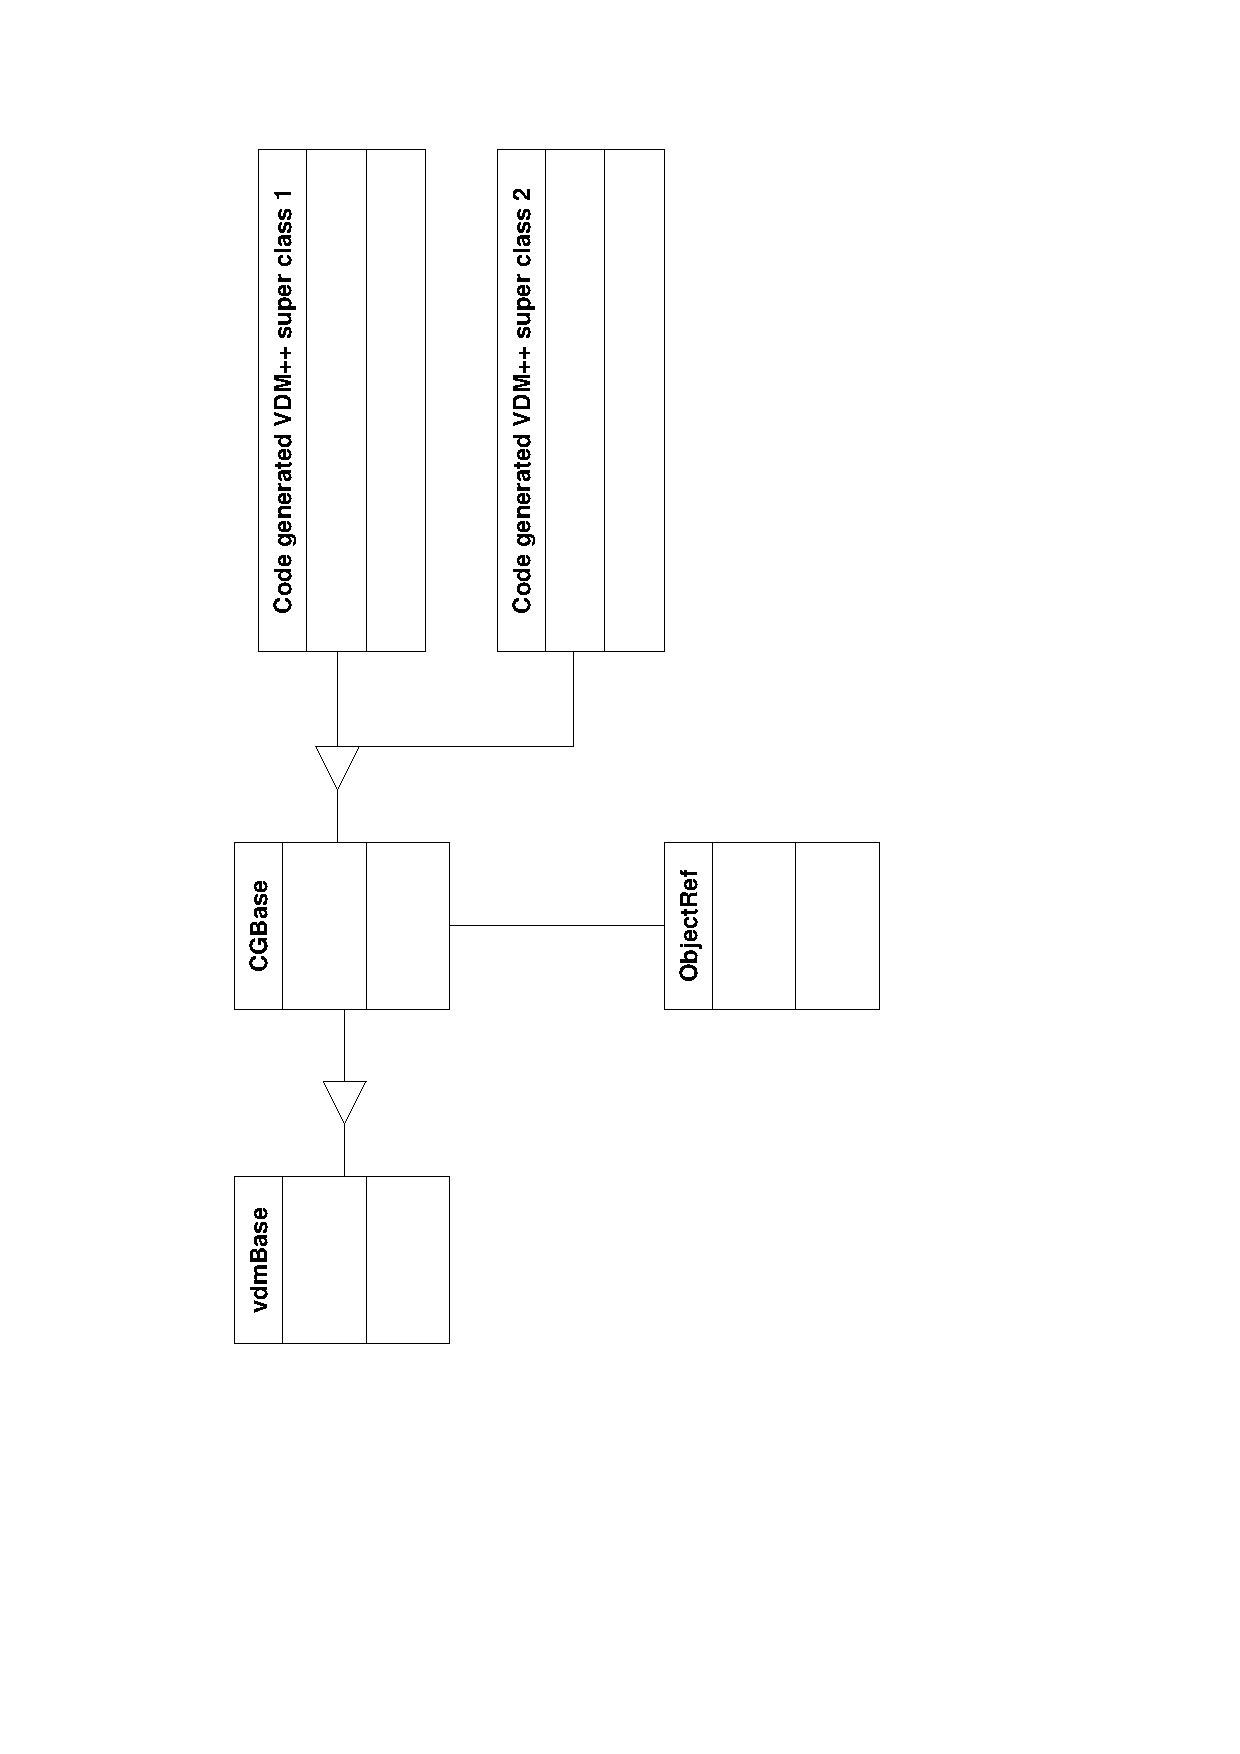
\includegraphics{cgbase}}}
    \caption{Relation between C++ classes \label{fig:cgb}}
  \end{center}
\end{figure}


%\insertfig{cgbase}{8cm}{Relation between C++
%  classes}{\label{fig:cgb}}



\subsection*{Examples}

Consider the following $VDM^{++}$ class:

\begin{verbatim}
class A

operations
  Test: () ==> nat
  Test()  == 
    let a = 10 + 10 in 
      return a

end A
\end{verbatim}

The following header file, {\tt A.h}, is generated by the {\it VDM++
  to C++ Code Generator\/}:

\begin{alltt}
{#ifndef _A_h}
{#define _A_h}

{#include <math.h>}
{#include "metaiv.h"}
{#include "cg.h"}
{#include "cg_aux.h"}
{#include "CGBase.h"}

class vdm_A : public virtual CGBase \{
public:
  virtual Int vdm_Test();

  vdm_A();
  virtual ~vdm_A() \{\}
\};

{#endif}
\end{alltt}

You can now use ObjectRef to implement object references of type {\tt A}
in the following way:

\begin{alltt}
{#include <iostream.h>}
{#include "A.h"}

int main ()
\{ 
  Sequence sq; Int i (10);
  ObjectRef cls1 (new vdm_A());
  ObjectRef cls2 (new vdm_A());

  sq.ImpAppend (i).ImpAppend (cls1).ImpAppend (cls2);

  wcout << VDM_A << " is the value of VDM_A" << endl;
  wcout << sq.ascii () << " is the value of sq" << endl;

  ObjectRef cls3 (sq[2]);
  if (cls3.MyObjectId () == VDM_A) \{ 
    vdm_A* cp = ObjGet_vdm_A(cls3);
    wcout << cp->vdm_Test ().ascii () << " is the result of Test ()" << endl;
    wcout << cls1 == cls2 << " is the result of cls1 == cls2" << endl;
    wcout << cls1 == cls3 << " is the result of cls1 == cls3" << endl;
  \}
  else
    wcout << "Something strange happened!" << endl;
\} 
\end{alltt}


\noindent The result of running this program is :

\begin{verbatim}
1 is the value of VDM_A
[ 10, @(1, 373776), @(1, 380808) ] is the value of sq
20 is the result of Test ()
0 is the result of cls1 == cls2
1 is the result of cls1 == cls3
\end{verbatim}



\subsection{Generic}

{\tt Generic} supports the following member functions:

\vspace{0.5cm}

\begin{description}
\item[{\tt Generic G}] \mbox{}\\
     Declares {\tt G} as a value of type {\tt Generic}. The value is
     an instance of GenericVal.

     Result type : {\bf void}

\item[{\tt Generic G(A)}] \mbox{}\\
     Declares {\tt G} as a value of type {\tt Generic} which value is equal to
     the value of {\tt A}.

     Result type : {\bf void}

\end{description}     

\section{SETs, SEQuences and MAPs}\label{templates}

For the types set, sequence and maps corresponding C++ templates
exists. These templates make it possible declare types with better
type information. Using these types it is possible to declare not only
a set but also which kind of value type the set can contain.

\subsection{SETs}

The {\tt SET} template is derived from the {\tt Set} class.

The {\tt SET} template support the constructor functions:

\begin{description}
\item[{\tt SET<A> St}] \mbox{}\\
Declares {\tt St} as a {\tt Set} of type {\tt A}. The value of {\tt
  St} is initialised to the empty set.

Result type: {\bf void}

\item[{\tt SET<A> St(St1)}] \mbox{} \\
Declares {\tt St} as a {\tt Set} of type {\tt A}. The value of {\tt
  St} is initialised to the value of {\tt St1}.

Result type: {\bf void}

\end{description}

In addition the same functions and operators that work on the {\tt
  Set} class are also declared for the {\tt SET} template.

\subsection{SEQuences}

The {\tt SEQ} template is derived from the {\tt Sequence} class.

The {\tt SEQ} template support the constructor functions:

\begin{description}
\item[{\tt SEQ<A> Sq}] \mbox{}\\
Declares {\tt Sq} as a {\tt Sequence} of type {\tt A}. The value of {\tt
  Sq} is initialised to the empty sequence.

Result type: {\bf void}

\item[{\tt SEQ<A> Sq(Sq1)}] \mbox{} \\
Declares {\tt Sq} as a {\tt Sequence} of type {\tt A}. The value of {\tt
  Sq} is initialised to the value of {\tt Sq1}.

Result type: {\bf void}

\end{description}

In addition the same functions and operators that work on the {\tt
  Sequence} class are also declared for the {\tt SEQ} template.

\subsection{MAPs}

The {\tt MAP} template is derived from the {\tt Map} class.

The {\tt MAP} template supports the constructor functions:

\begin{description}
\item[{\tt MAP<A,B> M}] \mbox{}\\
Declares {\tt M} as a {\tt Map} from type {\tt A} to {\tt B}. The value of {\tt
  M} is initialised to the empty map.

Result type: {\bf void}

\item[{\tt MAP<A, B> M(M1)}] \mbox{} \\
Declares {\tt M} as a {\tt Map} from type {\tt A} to {\tt B}. The value of {\tt
  M} is initialised to the value of {\tt M1}.

Result type: {\bf void}

\end{description}

In addition the same functions and operators that work on the {\tt
  Map} class are also declared for the {\tt MAP} template.



\section{Error messages} \label{error-messages}
When an error is detected by the library functions, an error number
along with a string describing the library function which detected the
error will be written to the m4err stream. Then the 'exit' function is
called to terminate the program.

The errors have been divided into two categories. User errors (U) are
errors that can appear under normal use of the library. An example
could be trying to extract an element from an empty set.

Internal errors (I) are more severe errors. These errors should not appear
under normal use of the libraries.

\vspace{0.5cm}
\noindent

\begin{tabular}{|r|l|p{5.5cm}|c|} \hline
{\em No.} & {\em Symbolic name} & {\em Description} 
           & {\em Error type} \\ \hline \hline
1   & {\tt ML\_CONFLICTING\_RNGVAL} & Insert a key in a map which already exists
      with a different range value&U\\
2   & {\tt ML\_NOT\_IN\_DOM} & Applying a map with a key which is not in domain&U\\
3   & {\tt ML\_CAST\_ERROR} & Generic casted to wrong type&U\\
4   & {\tt ML\_INDEX\_OUT\_OF\_RANGE} & Index out of range in sequence, tuple
      or record function&U\\
5   & {\tt ML\_OP\_ON\_EMPTY\_SEQ} & Illegal function on empty sequence&U\\
6   & {\tt ML\_OP\_ON\_EMPTY\_SET} & Illegal function on empty set&U\\
7   & {\tt ML\_NOT\_IN\_SET} & Tried to remove non-existing
                               element&U\\
8   & {\tt ML\_ASSIGN\_ERROR} & Tried to assign two variables of
                                different types&U\\
9   & {\tt ML\_TRAVERSE\_CONFLICT} & Error detected while evaluating
                                    the member function next&I\\
10  & {\tt ML\_HD\_ON\_EMPTY\_SEQUENCE} & Tried to take hd on an empty
                                          sequence&U\\                      
11  & {\tt ML\_TL\_ON\_EMPTY\_SEQUENCE} & Tried to take tl on an empty
                                          sequence&U\\
12  & {\tt ML\_RANGE\_ERROR} & Index out of range for tuple or record&U\\                                                   
13  & {\tt ML\_ZERO\_REFCOUNT} & Zero refcount detected&I\\
14  & {\tt ML\_NULL\_REF} & Zero pointer reference&I\\\hline
15  & {\tt ML\_DIV\_BY\_ZERO} & Division by zero. & U \\ \hline 
\end{tabular}


\bibliographystyle{iptes}
\bibliography{ifad}

 
\appendix
\section{Files} \label{files}
The interface to the VDM C++ Library consists of the following
files:

\begin{description}
\item[metaiv.h] is the header file containing the prototypes of all the
  type specific functions described in section \ref{specific-op}.
   
\item[libvdm.a] is a library archive containing the implementation
     of all the functions described in this document.
\end{description}
\end{document}
